\documentclass[a4paper, 12pt]{article}
\usepackage{comment} % enables the use of multi-line comments (\ifx \fi) 
\usepackage{lipsum} %This package just generates Lorem Ipsum filler text. 
\usepackage{fullpage} % changes the margin
\usepackage[utf8]{inputenc}
\usepackage{algorithm}
\usepackage{algorithmicx}
\usepackage{algpseudocode}
\usepackage{graphicx}
\usepackage{mathtools}
\usepackage{amsmath}


\begin{document}
%Header-Make sure you update this information!!!!
\noindent
\large\textbf{Documentação TP3} \hfill \textbf{Ícaro Harry} \\
\normalsize AEDS3 \hfill  Matrícula: 2014033050\\


\section{Introdução}
\paragraph{}
O trabalho proposto no TP3 foi a simulação de um jogo de Cassino, onde dada uma sequência de números, deveríamos determinar o maior valor possível de se obter apenas somando ou subtraindo os números. Para ganhar o jogo, era necessário que o valor obtido fosse maior do que um limite mínimo. Além disse as operações não poderiam ultrapassar o limite inferior de 0 e o limite superior dado em cada instância do problema.
\paragraph{}
O principal desafio do TP era desenvolver uma estratégia de força bruta e melhorá-la através de um algoritmo de Programação Dinâmica ou Guloso. Além disso, deveríamos ecolher uma das duas abordagens e desenvolver um algoritmo paralelizado para o problema.

\section{Solução do Problema}
\paragraph{}
Como abordado na seção anterior, para resolver o problema, primeiro deveríamos desenvolver uma solução de força bruta e depois escolher entre uma abordagem Gulosa ou uma abordagem de Programação Dinâmica para melhorar o problema.

\subsection{Força bruta}
\paragraph{}
A estratégia de força bruta pode ser facilmente implementada de maneira recursiva, percorrendo todas as possibilidades possíveis de soma ou subtração, como demonstrado na figura abaixo:
\begin{figure}[!h]
\centering
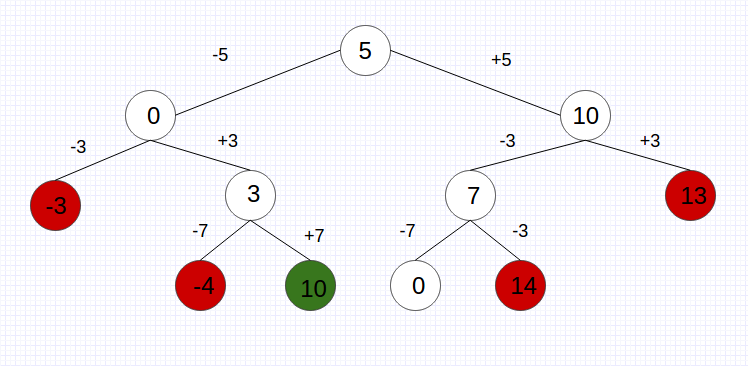
\includegraphics[scale=0.4]{sum.png}
\caption{Toy example}
\end{figure}

\paragraph{}
O exemplo acima demonstra o Toy example, onde iniciando com o valor 5, devemos utilizar 5, 3 e 7 para obter a maior soma possível, dentro do limite máximo de 10. Então o algoritmo testa todas as possibilidades, podando quando elas ultrapassam o limite de 0 ou 10, o que está destacado em vermelho na figura. No último passo da recursão, o algoritmo busca o maior valor de todos, no caso 10, que está destacado em verde.

\paragraph{}
O algoritmo implementado de maneira recursiva é o seguinte:


\begin{algorithm}
\caption{Brute Force}
\begin{algorithmic}
\Function{playGame}{$seqSize$, $sum$, $limit$, $sequence$, $element$, $k$, $bigger$}
	\If{($sum$ + $element$ minor or equal $limit$ and $k$ minor than $seqSize$)}
		\State playGame($seqSize$, $sum$ + $element$, $limit$, $sequence$, $sequence[k + 1]$, $k$ + 1, $bigger$);    
    		
	\EndIf
	\If{($sum$ - $element$ bigger or equal $0$ and $k$ minor than $seqSize$)}
		\State playGame($seqSize$, $sum$ - $elemnt$, $limit$, $sequence$, $sequence[k + 1]$, $k$ + 1, $bigger$);    
    		
	\EndIf 
	\If{$k$ == $seqSize$}
		\State $bigger$ = $sum$ bigger than $bigger$ ? $sum$ : $bigger$;    
    		
	\EndIf  
    
\EndFunction
\end{algorithmic}
\end{algorithm}




\subsection{Programação Dinâmica ou Algoritmo Guloso?}
\paragraph{}
É simples determinar qual abordagem serve para obter uma solução ótima para o problema. Sabemos que um algoritmo guloso caminha para a solução ótima tomando sempre a melhor decisão local. No problema em questão, a escolha local vai ser sempre somar ou subtrair o número X do número Y. Porém é fácil perceber que, tomando uma decisão ótima do maior número obtido válido, entre a soma e a subtração, não nos permite eliminar a outra possibilidade, pois o próximo valor poderá tornar a solução escolhida inválida, já que ele pode tornar a soma maior do que o limite superior ou menor do que 0. É possível enxergar isso no Toy Example desenhado acima. A escolha ótima local levaria para o lado direito da árvore de possibilidades, porém o resultado ótimo está do outro lado.

\paragraph{}
Sendo assim, para resolver o problema de maneira ótima e, ao mesmo tempo, melhorar a performance do algoritmo de força bruta, escolhi utilizar uma abordagem de Programação Dinâmica.

\subsubsection{Resolução com Programação Dinâmica}
\paragraph{}
O algoritmo de Programação Dinâmica utiliza uma matriz para marcar os valores das somas obtidas em cada passo. A tabela abaixo ilustra o Toy Example:

\begin{figure}[!h]
\centering
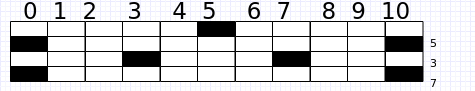
\includegraphics[scale=0.4]{pd.png}
\caption{Toy example}
\end{figure}
\paragraph{}
Cada linha da matriz corresponde a um estado das somas, sendo o estado inicial fornecido na entrada. As colunas representam os possíveis valores no intervalo entre 0 inclusive e X inclusive. Dessa maneira, a cada passo do algoritmo, marca-se os próximos valores somados. Se a soma ultrapassar os limites, não é feito nada. Ao final do algoritmo, o resultado estará na última linha da matriz e corresponderá ao índice da última posição marcada.

\begin{algorithm}
\caption{Programação Dinâmica}
\begin{algorithmic}
\Function{playGame}{$seqSize$, $sum$, $limit$, $sequence$}
    \State $m$ = createMatrix($seqSize + 1$, $limit + 1$);
	\State $m[0][sum]$ = true;    
    \For{$i$ = 0; $i$ minor than $seqSize$; $i$++}
		\For{$j$ = 0; $i$ minor or equal $limit$; $j$++}
			\If{$m[i][j]$}
				\If{($j$ + $sequence[i]$ minor or equal $limit$)}
					\State $m[i+1][j + sequence[i]]$ = true;
				\EndIf
				\If{($j$ + $sequence[i]$ bigger or equal $0$)}
					\State $m[i+1][j - sequence[i]]$ = true;
				\EndIf
			\EndIf
		\EndFor
    \EndFor
    \For{$i$ = $limit$; $i$ bigger or equal $0$; $i$--}
		    \If{$m[seqSize][i]$}
		    	\State return $i$;
		    \EndIf
    \EndFor
    \State return $-1$;
\EndFunction
\end{algorithmic}
\end{algorithm}


\section{Análise Teórica do Custo Assintótico de Tempo}
\paragraph{}
O problema proposto, na abordagem por força bruta, testa todas as possibilidades possíveis de soma e subtração de cada elemento, apenas podando aquelas somas que ultrapassam os limites estabelecidos. Dessa maneira, como podemos observar na figura 1, a cada passo do algoritmo, ou seja, a cada novo número para se somar e subtrair, multiplica-se por dois os números que devem ser testados, o que nos leva a uma complexidade de {\(O(2^S)\)}, sendo S o número da sequência dada na entrada.

\paragraph{}
Podemos observar que o algoritmo de Programação Dinâmica reduz consideravelmente a complexidade em relação ao algoritmo de força bruta. Para chegar ao resultado final, deve-se percorrer a matriz, linha por linha, checando se cada posição está marcada ou não. Ou seja, a complexidade de tempo é dada pelo tamanho da matriz a ser percorrida, no caso é S + 1 por X + 1, sendo S o tamanho da sequência dada e X o limite superior dado. Para encontrar o maior resultado na última linha da matriz, deve-se percorrê-la de trás para frente, o que nos dá uma complexidade de O((S+1) * (X+2)) = O(S*X).


\section{Análise Teórica do Custo Assintótico de Espaço}
\paragraph{}
O algoritmo de força bruta utiliza apenas um vetor com os números que compõem a sequência dada na entrada, dessa maneira, a complexidade de espaço é O(S).
\paragraph{}
Já a programação dinâmica, claramente troca computação por espaço, para evitar de se percorrer todas as {\(2^S)\)} possibilidades, deve-se criar uma matriz de tamanho S + 1 por X + 1. Sendo assim, a complexidade de espaço é O(S*X).


\section{Análise Experimental do Custo Assintótico}
\paragraph{}
Para verificar o custo assintótico, realizei testes utilizando entradas que aumentavam de 1 em 1, como demonstrado no algoritmo abaixo. Para medi-los utilizei a função clock da biblioteca time.h.
\begin{algorithm}
\caption{Testes}
\begin{algorithmic}
\Function{test}{}
    \For{$i$ = 0; $i$ minor than $limit$; $i$++}
		\For{$j$ = 0; $j$ minor than $i$; $j$--}
		    \State $sequence[j]$ = 1;
    	\EndFor
    	\State $begin$ = clock();
        \State playGame($i$, $0$, $limit$, $30$, $sequence$);
        \State $end$ = clock();
        \State $timeSpent$ = (double)($end$ - $begin$) / $CLOCKS_PER_SEC$;
    \EndFor
\EndFunction
\end{algorithmic}
\end{algorithm}

\paragraph{}
Os resultados obtidos estão descritos nos seguintes gráficos:

\begin{figure}[!h]
\centering
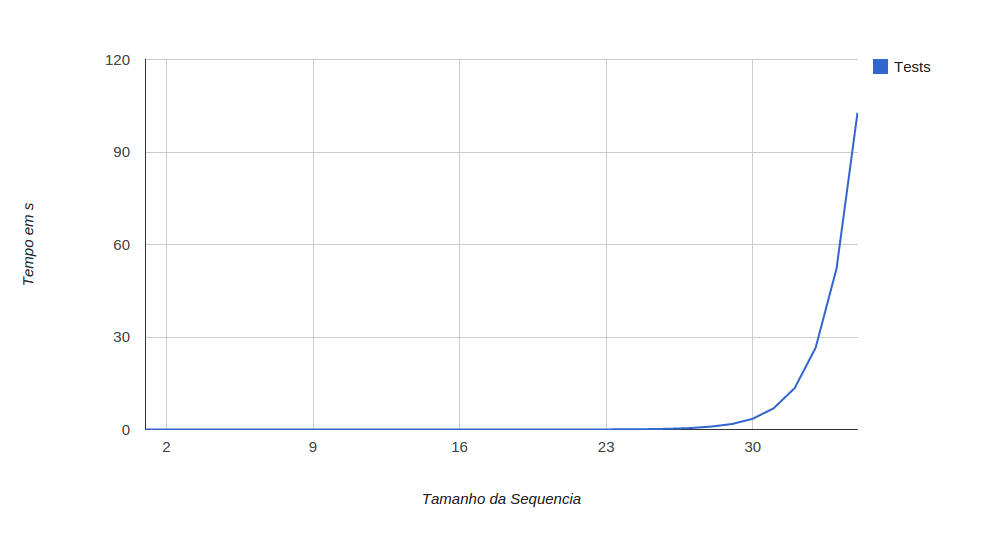
\includegraphics[scale=0.4]{graficoBF.png}
\caption{Força bruta com entradas de 1 a 35}
\end{figure}

\begin{figure}[!h]
\centering
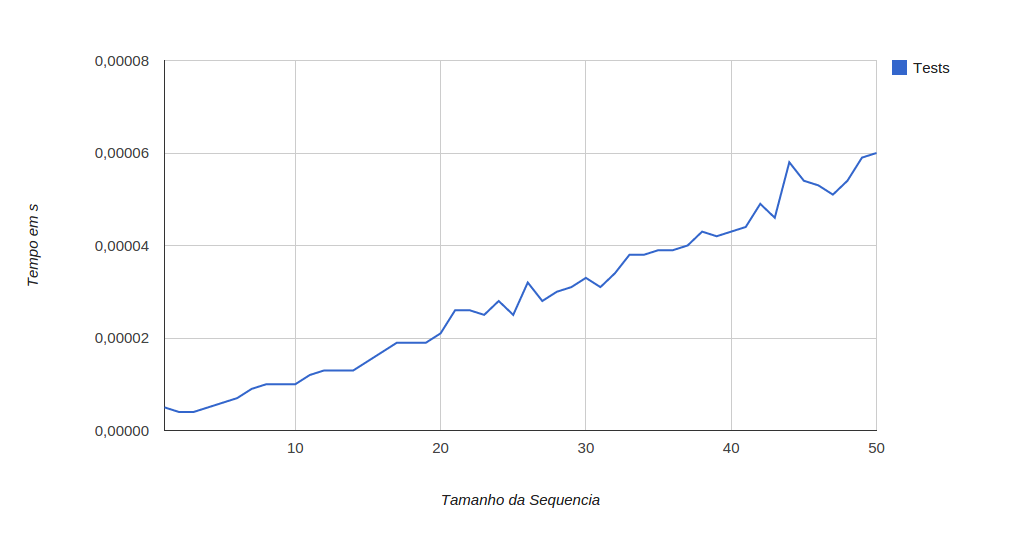
\includegraphics[scale=0.4]{graficoPD.png}
\caption{Programação Dinâmica com entradas de 1 a 50}
\end{figure}

\section{Conclusão}
\paragraph{}
Pude concluir com o presente Trabalho Prático que problemas que aparentemente possuem natureza exponencial, podem ser resolvidos com soluções muito mais eficientes utilizando Programação Dinâmica.


\end{document}
